\documentclass[12pt]{article}

\author{Ethan Khai Dang}
\date{Fall 2023}

% Packages
\usepackage[T1]{fontenc} % Some font fixes
\usepackage{amsmath, amssymb, amsthm} % Allows extra math commands
\usepackage{listings} % Allows importing code
\usepackage{url}
\usepackage{hyperref}
\usepackage{subcaption} % Helps with figures
\usepackage{graphicx} % Allows including images
\usepackage[dvipsnames,table]{xcolor} % Helps with manipulating colors
\usepackage[legalpaper, margin=1in]{geometry} % Adjusts page margins
\usepackage{tikz}
\usetikzlibrary{automata, positioning, arrows, shapes}

% Settings for portfolio
\title{Secure Drop Project: Codebase and Documentation}
\setcounter{tocdepth}{2}

% Formatting style for code
\definecolor{backcolour}{rgb}{0.92,0.92,0.90}
\lstdefinestyle{pythoncode}{
    language=Python,
    basicstyle=\ttfamily\footnotesize,
    commentstyle=\color{Green},
    tabsize=4,
    columns=flexible,
    keepspaces=true,
    numbers=left,
    keywordstyle=\color{Blue},
    stringstyle=\color{Maroon},
    showstringspaces=false,
    backgroundcolor=\color{backcolour},
    frame=single,
    breaklines=true
}
\lstset{style=pythoncode}

% Get images from figures directory
\graphicspath{ {./figures/} }

\begin{document}

\maketitle
\tableofcontents

\newpage

\section{Pretense}
During the Fall semester of 2023, I was building this project as part of a course in computer security towards my Cybersecurity concentration of Computer Science.
I learned a lot about secure communication and how to implement it in a real-world scenario as part of a Intro to Computer Security course at the University of Massachusetts - Lowell. 
The importance of secure communication and how it can be used to protect sensitive information.
Through work with Sashank Narain, I was able to get access to concepts like Pretty Good Privacy (PGP) and how it can be used to secure communication, as well as TLS schemes and how they can be used to secure communication over the internet.

In the class, we discussed several vulnerabilities related to mobile devices, a topic Sashank was researching at the time.
The example he gave was about Apple's AirDrop feature, which allows users to share files between Apple devices. However, the feature had a vulnerability that could allow attackers to obtain a user's phone number and email address. This vulnerability was due to the lack of encryption in the AirDrop feature, which made it possible for attackers to intercept the data being transferred.

Providing man-in-the-middle attacks, attackers could intercept the data being transferred between devices and obtain sensitive information. This vulnerability highlighted the need for this project and what it aims to achieve.
Through this context, the project was built on the premise of secure communication between users over a network. It assumes that users have access to the necessary certificates and keys for establishing secure connections. The project aims to provide a secure and user-friendly environment for transferring files and messages while ensuring data integrity and confidentiality.

It's easy to see how Malicious actors can now leverage sophisticated tools and techniques that require less technical expertise to execute complex attacks. This trend is particularly evident in the realm of mobile device security, where vulnerabilities like the one found in Apple's AirDrop can be exploited with relative ease.

While it may seem like a minor issue, it underscores a broader problem: the increasing reliance on insecure communication protocols. As more and more devices become interconnected, the attack surface expands exponentially. Malicious actors can exploit these vulnerabilities to gain unauthorized access to sensitive information, financial data, and personal communications.

To address this growing threat, it's important to understand this topic and addressing it at a basic level to develop basic understanding of network security. By implementing robust encryption techniques, such as PGP and TLS, we can safeguard sensitive information very easily and efficiently. Staying informed about the latest security threats and vulnerabilities is crucial.

It is essential to adopt a proactive approach to security. By prioritizing secure communication, staying informed about emerging threats, and regularly updating software and systems, we can safeguard our digital assets and protect ourselves from harm. With this in mind, the project to make a "better" AirDrop serves to make me informed and learn about these simple protocols and schemes and really have a fundamental understand of security as someone approaching this field.

\newpage
\section{Project Structure}
\begin{verbatim}
.env
bin/
    ca.crt
    ca.key
    ca.sh
    certs/
        client_certs.sh
downloads/
example.txt
README.md
requirements.txt
run.sh
secure_drop.py
src/
    globals.py
    network/
        __init__.py
        broadcast.py
        contact.py
        ndata.py
        tcp.py
    nglobals.py
    run.py
    secure_shell/
        __init__.py
        login.py
        registration.py
        sd_shell.py
    utility/
        __init__.py
        crypt.py
        data.py
        input.py
        quit.py
users.json
\end{verbatim}

\subsection{Python Packages and Modules}
Python, as an interpreted language, organizes code into packages and modules to promote modularity and reusability. A module is a single file containing Python code, while a package is a directory containing multiple modules and an \texttt{\_\_init\_\_.py} file to indicate that the directory is a package. This structure allows for better organization of code, making it easier to manage and maintain.

For the Secure Drop project, I chose to set up the project as a series of packages to logically separate different functionalities. This modular approach ensures that each component of the project is self-contained and can be developed, tested, and maintained independently. The main packages in the project are:


\newpage

\section{Project Functionalities}
Aptly named "Secure Drop", this application is built to be a Secure File Transfer Protocol (SFTP) Command Line Interface (CLI).
Using Python and relying on several external libraries, such as PyCryptodome for cryptographic operations and OpenSSL for certificate management, was paramount in understanding the higher-level concepts being taught in the class.
The main functionalities of the project include:

\subsection{Certificate and Key Management}
Scripts and files for generating and managing RSA keys and X.509 certificates are essential for establishing secure communication channels. These components ensure data authenticity and prevent unauthorized access.

\subsection{Cryptographic Utilities}
Functions for encryption, decryption, hashing, and key generation are crucial for ensuring the security and integrity of data within the Secure Drop project. These utilities provide the necessary tools to implement secure communication protocols.

\subsection{Secure Shell}
A command-line interface for client interactions, including login, registration, and secure file transfer, provides a user-friendly interface for interacting with the Secure Drop system. This shell manages user sessions and facilitates secure file transfers.

\subsection{Control Flow Management}
Mechanisms to limit message processing rates and protect against flooding DoS attacks are implemented to ensure the system's stability and security. These controls prevent denial-of-service attacks by capping the message processing rate.

\subsection{Session Management}
Unique session tokens for each login session ensure secure and authenticated user interactions. This mechanism prevents impersonation and ensures that only authorized users can access the system.

\newpage

\section{Certificate and Key Management}
The project includes scripts and files for generating and managing certificates and keys. In reality, these would be managed by a trusted Certificate Authority (CA).

\subsection{Pretty Good Privacy (PGP)}
Typically, PGP is used to secure communication between users. However, in this project, we use OpenSSL to generate certificates and keys for secure communication.
In reality, PGP would be used to encrypt and decrypt messages between users, as shown in Figure \ref{fig:pgp_scheme}.
For ease of access and simple demonstration however, we just use OpenSSL to generate a certificate authority on file. The certificate authority is then used to sign certificates for secure communication.
Using this larger authority however allows users to cross check certificates issued to it from other users, ensuring that the certificate is valid and secure.

\begin{figure}[h]
    \centering
    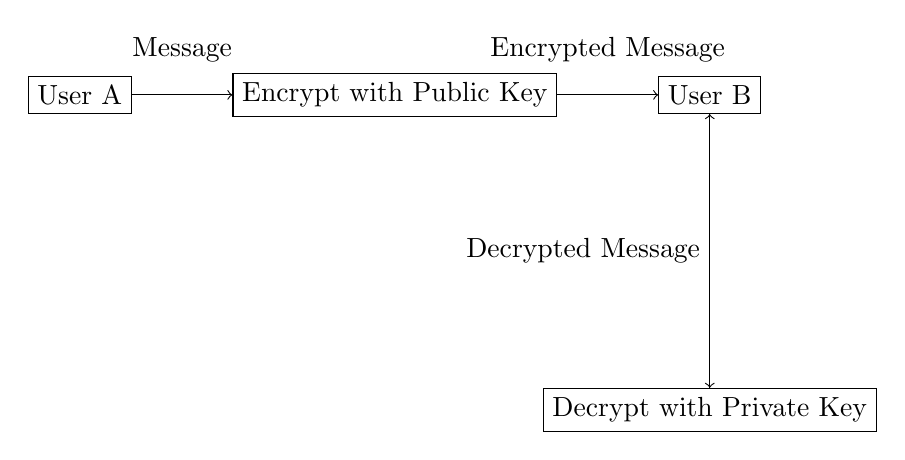
\begin{tikzpicture}[node distance=6cm, auto]
        % Nodes
        \node (userA) [draw, rectangle] {User A};
        \node (encrypt) [draw, rectangle, right of=userA, node distance=4cm] {Encrypt with Public Key};
        \node (userB) [draw, rectangle, right of=encrypt, node distance=4cm] {User B};
        \node (decrypt) [draw, rectangle, below of=userB, node distance=4cm] {Decrypt with Private Key};
        
        % Arrows
        \draw[->] (userA) -- node[above, pos=0.5, yshift=0.3cm] {Message} (encrypt);
        \draw[->] (encrypt) -- node[above, pos=0.5, yshift=0.3cm] {Encrypted Message} (userB);
        \draw[->] (userB) -- (decrypt);
        \draw[->] (decrypt) -- node {Decrypted Message} (userB);
    \end{tikzpicture}
    \caption{PGP Scheme for Secure Communication}
    \label{fig:pgp_scheme}
\end{figure}

\subsection{Certificate File}
\lstinputlisting[language=, caption=Certificate File]{bin/ca.crt}

\subsection{Key File}
\lstinputlisting[language=, caption=Key File]{bin/ca.key}

\subsection{Shell Script for Certificate Authority}
The shell script for the Certificate Authority (CA), located at ca.sh, generates a new RSA private key and a self-signed X.509 certificate, which are saved as ca.key and ca.crt respectively.
This script is crucial for establishing a trusted CA within the Secure Drop project, as it provides the root of trust for all client certificates.
By signing client certificates with this CA, the project ensures that all communications are authenticated and encrypted, thereby maintaining data integrity and preventing unauthorized access.
However, it should be noted that in a real-world scenario, the CA would be managed by a trusted third party, such as a Certificate Authority (CA) or a Public Key Infrastructure (PKI) provider.
Having a CA on file is a simple demonstration of how certificates and keys are managed in a secure communication system.

\lstinputlisting[language=bash, caption=Shell Script for Certificate Authority]{bin/ca.sh}

\begin{itemize}
    \item Certificate File (\texttt{bin/ca.crt}) containing the trusted certificate authority.
    \item Key File (\texttt{bin/ca.key}) used for signing certificates.
    \item Shell Script for Certificate Authority (\texttt{bin/ca.sh}) for managing certificates.
\end{itemize}

These sections are crucial for establishing secure communication channels. Having a trusted certificate authority and managing keys ensures data authenticity and prevents unauthorized access.

\newpage

\section{Utility Functions}
The utility functions are defined in the \texttt{src/utility} directory. In general, there were a lot of requirements for the project as previously mentioned.
The utility functions are essential for handling cryptographic operations, data management, and user interactions within the Secure Drop project, mostly since they handled application-level operations.
These operations were mostly used on crude data, such as user input, file management, and cryptographic operations. To tackle the handling and conversion in interactions between these data points, utility functions were split into three sections.

\subsection{Cryptography Functions}
\lstinputlisting[language=Python, caption=Cryptography Functions]{src/utility/crypt.py}

The cryptography functions in the utility module, are essential for ensuring the security and integrity of data within the Secure Drop project. These functions handle various cryptographic operations such as encryption, decryption, hashing, and key generation. By utilizing these functions, the project can securely encrypt files and messages before transmission, ensuring that only authorized recipients can decrypt and access the data. Additionally, hashing functions are used to verify data integrity, ensuring that the data has not been tampered with during transmission. These cryptographic utilities are foundational to the project's security architecture, as they provide the necessary tools to implement secure communication protocols. Later in the project, these functions are used in the secure shell module for encrypting user credentials during login and registration processes, as well as in the network module for encrypting and decrypting messages exchanged between clients. This ensures that all data transferred within the Secure Drop system is protected against unauthorized access and tampering, maintaining the confidentiality and integrity of the information.

\subsection{Data Management Functions}
\lstinputlisting[language=Python, caption=Data Management Functions]{src/utility/data.py}

The data management functions in the utility module, are crucial for handling and manipulating data within the Secure Drop project. These functions provide essential operations such as reading from and writing to files, parsing and formatting data, and managing user information. By utilizing these functions, the project ensures that data is consistently and efficiently processed, stored, and retrieved. For example, these functions are used to manage user credentials, store encrypted messages, and handle file transfers. Later in the project, the data management functions are employed in the secure shell module to manage user registration and login information, ensuring that user data is securely stored and easily accessible when needed. Additionally, in the network module, these functions facilitate the handling of data packets and message exchanges between clients, ensuring that data is correctly formatted and transmitted. Overall, the data management functions are integral to the project's ability to handle and process data securely and efficiently, maintaining the integrity and availability of the information within the Secure Drop system.

\subsection{Utility Module Initialization}
\lstinputlisting[language=Python, caption=Utility Module Initialization]{src/utility/__init__.py}

\begin{itemize}
    \item Cryptography Functions (\texttt{src/utility/crypt.py}) for encryption, decryption, hashing, and key generation.
    \item Data Management Functions (\texttt{src/utility/data.py}) for data manipulation and storage.
    \item Utility Module Initialization (\texttt{src/utility/\_\_init\_\_.py}) to import and configure utility functions.
\end{itemize}

Utility functions are essential building blocks for cryptographic operations within the project. They provide the core functionalities for secure data handling.

\newpage

\section{Network Functions}
The network functions are defined in the \texttt{src/network} directory. These functions are crucial for enabling communication between users within the Secure Drop application. The network module employs two different types of protocols: TCP (Transmission Control Protocol) and UDP (User Datagram Protocol) to discover and maintain connections with users.

\subsection{TCP and UDP Protocols}
TCP and UDP are fundamental protocols in the Internet Protocol (IP) suite, each serving different purposes. TCP, developed in the 1970s as part of the ARPANET project, is a connection-oriented protocol that ensures reliable and ordered delivery of data between applications. It establishes a connection before data transfer and uses acknowledgments to confirm receipt of packets, making it suitable for applications where data integrity is critical.

On the other hand, UDP, also developed in the 1980s, is a connectionless protocol that allows for faster data transmission by sending packets without establishing a connection or waiting for acknowledgments. This makes UDP ideal for applications where speed is more critical than reliability, such as real-time video streaming or online gaming.

\subsection{Discovery and Pinging Mechanism}
In the Secure Drop application, UDP is used for discovering users on the network. The \texttt{broadcast.py} file contains functions that send broadcast messages to all devices on the local network, allowing the application to discover other users running the Secure Drop application. This discovery mechanism leverages the speed and efficiency of UDP to quickly identify available users.

Once users are discovered, TCP is used to establish and maintain reliable connections between them. The \texttt{tcp.py} file contains functions that handle the establishment of TCP connections, ensuring that data is transmitted reliably and in order. This is crucial for file transfers and secure messaging, where data integrity and order are paramount.

\subsection{TLS Scheme}
To further enhance security, a TLS (Transport Layer Security) scheme is implemented within the TCP connections. TLS is a cryptographic protocol designed to provide secure communication over a computer network. It evolved from the SSL (Secure Sockets Layer) protocol developed by Netscape in the mid-1990s.

In the Secure Drop application, the TLS scheme is implemented to encrypt data transmitted over TCP connections, ensuring that sensitive information such as user credentials and file contents are protected from eavesdropping and tampering. The TLS scheme involves the following steps:
\begin{enumerate}
    \item \textbf{Handshake}: The client and server exchange cryptographic keys and agree on encryption algorithms.
    \item \textbf{Encryption}: Data is encrypted using symmetric encryption algorithms, ensuring confidentiality.
    \item \textbf{Integrity}: Message integrity is ensured using hashing algorithms, preventing tampering.
    \item \textbf{Authentication}: The server's identity is authenticated using digital certificates, ensuring that the client is communicating with a trusted server.
\end{enumerate}

The \texttt{tcp.py} file contains functions that handle the TLS handshake and encryption processes, ensuring that all data transmitted over TCP connections is secure.


\subsection{Network Initialization}
\lstinputlisting[language=Python, caption=Network Initialization]{src/network/__init__.py}

\subsection{Broadcast Functions}
\lstinputlisting[language=Python, caption=Broadcast Functions]{src/network/broadcast.py}

\subsection{Contact Functions}
\lstinputlisting[language=Python, caption=Contact Functions]{src/network/contact.py}

\subsection{Network Data Functions}
\lstinputlisting[language=Python, caption=Network Data Functions]{src/network/ndata.py}

\subsection{TCP Functions}
\lstinputlisting[language=Python, caption=TCP Functions]{src/network/tcp.py}

\begin{itemize}
    \item Network Initialization (\texttt{src/network/\_\_init\_\_.py}) to set up network connections.
    \item Broadcast Functions (\texttt{src/network/broadcast.py}) for sending messages to multiple recipients.
    \item Contact Functions (\texttt{src/network/contact.py}) for managing communication with other users.
    \item Network Data Functions (\texttt{src/network/ndata.py}) for handling network data transmission and reception.
    \item TCP Functions (\texttt{src/network/tcp.py}) for managing TCP communication protocols.
\end{itemize}

Network functions enable communication within the Secure Drop system. They allow users to securely exchange messages and files over the network.

\newpage

\section{Secure Shell}
This component of the Secure Drop project provides a command-line interface (CLI) for user interactions, including login, registration, and secure file transfer.
As part of the course requirements set by my professor, we were tasked with creating a secure shell for our project. The goal was to provide a user-friendly interface that allows users to interact with the Secure Drop system securely. This shell needed to handle user authentication, manage sessions, and facilitate secure file transfers.
At the same time, the shell needed to be intuitive and easy to use, ensuring that users could navigate the system with minimal technical knowledge.

\subsection{Implementation}
To implement the secure shell, I leveraged the convenience and power of Python libraries. Python's extensive standard library and third-party modules made it possible to create a robust and secure shell with relative ease. The directory contains the following key components:

\begin{itemize}
    \item \textbf{Secure Shell Initialization:} (\texttt{src/secure\_shell/\_\_init\_\_.py}) This file sets up the secure shell environment, initializing necessary configurations and dependencies.
    \item \textbf{Login Functions:} (\texttt{src/secure\_shell/login.py}) These functions handle user authentication, verifying credentials and establishing secure sessions.
    \item \textbf{Registration Functions:} (\texttt{src/secure\_shell/registration.py}) These functions manage user registration, securely storing user credentials and creating new accounts.
    \item \textbf{Secure Shell Functions:} (\texttt{src/secure\_shell/sd\_shell.py}) This file contains the core functions that handle user interactions within the secure shell, including commands for file transfer, session management, and communication.
\end{itemize}

\subsection{Why Python?}
Creating a secure shell from scratch using traditional CLI tools would have been incredibly challenging and time-consuming. Python's libraries, such as \texttt{argparse} for command-line argument parsing, \texttt{getpass} for secure password input, and \texttt{cryptography} for encryption and decryption, provided the necessary functionality to build a secure and user-friendly shell efficiently. Additionally, Python's readability and ease of use allowed for rapid development and debugging, ensuring that the shell met the project requirements within the given timeframe.

\subsection{Benefits of the Secure Shell}
The secure shell provides several benefits to the Secure Drop project:
\begin{itemize}
    \item \textbf{User-Friendly Interface:} The shell offers a simple and intuitive interface for users to interact with the system, making it accessible even to those with limited technical knowledge.
    \item \textbf{Secure Authentication:} By handling user login and registration securely, the shell ensures that only authorized users can access the system.
    \item \textbf{Session Management:} The shell manages user sessions, maintaining security and preventing unauthorized access.
    \item \textbf{Secure File Transfer:} The shell facilitates secure file transfers, encrypting data to protect it from eavesdropping and tampering.
\end{itemize}

\subsection{Code Snippets}
\subsubsection{Secure Shell Initialization}
\lstinputlisting[language=Python, caption={Secure Shell Initialization}]{src/secure_shell/__init__.py}

\subsubsection{Login Functions}
\lstinputlisting[language=Python, caption={Login Functions}]{src/secure_shell/login.py}

\subsubsection{Registration Functions}
\lstinputlisting[language=Python, caption={Registration Functions}]{src/secure_shell/registration.py}

\subsubsection{Secure Shell Functions}
\lstinputlisting[language=Python, caption={Secure Shell Functions}]{src/secure_shell/sd_shell.py}

\newpage

\section{Project Dependencies}
The project dependencies are listed in the \texttt{requirements.txt} file.

\lstinputlisting[language=, caption=Project Dependencies]{requirements.txt}

\subsection{Dependency Details}

\subsubsection{PyCryptodome}
\textbf{History:} PyCryptodome is a self-contained Python package of low-level cryptographic primitives. It was created as a fork of the PyCrypto library, which had not been updated for several years at the time of its inception. PyCryptodome aims to provide a more secure and up-to-date alternative to PyCrypto, with additional features and improvements.

\textbf{Reason for Selection:} PyCryptodome was chosen for its comprehensive suite of cryptographic functions, including encryption, decryption, hashing, and key generation. These functions are essential for ensuring the security and integrity of data within the Secure Drop project. The library's ease of use and active maintenance make it a reliable choice for implementing cryptographic operations.

\subsubsection{OpenSSL}
\textbf{History:} OpenSSL is a robust, full-featured open-source toolkit implementing the Secure Sockets Layer (SSL) and Transport Layer Security (TLS) protocols. It also includes a general-purpose cryptography library. OpenSSL has been widely used since its inception in 1998 and is maintained by the OpenSSL Project.

\textbf{Reason for Selection:} OpenSSL was chosen for its extensive support for SSL/TLS protocols and its ability to generate and manage X.509 certificates and RSA keys. These features are crucial for establishing secure communication channels and managing certificates within the Secure Drop project. OpenSSL's reliability and widespread adoption make it a trusted choice for cryptographic operations.

\newpage

\section{Project Overview}

The Secure Drop project serves as a tangible example of how robust cybersecurity practices can be implemented to safeguard sensitive information. By delving into the intricacies of secure communication and data protection, I gained a deeper appreciation for the importance of these concepts in today's technical landscape.

The project's success underscores the significance of adhering to fundamental cybersecurity principles, such as the CIA triad: Confidentiality, Integrity, and Availability. By ensuring that data remains private, accurate, and accessible to authorized users, we can mitigate the risks associated with data breaches and unauthorized access.

Beyond the specific technical implementations, it highlights the broader implications of cybersecurity and privacy. As technology continues to advance, so too do the threats to digital security. By understanding the underlying principles and best practices, it helps anyones understanding of informational systems as a whole.

The project overview is provided in the \texttt{README.md} file.
\lstinputlisting[language=, caption=Project Overview]{README.md}

\end{document}